
% Figures Related to Trust Management
%%%%%%%%%%%%%%%%%%%%%%%%%%%%%%%%%%%%%

\newcommand{\tmstructfig}
{
\begin{fpfig}[t]{Structure of an Authorization Decision}{figure-tmstruct}
\vspace{2mm}
\begin{tabular}{cc}
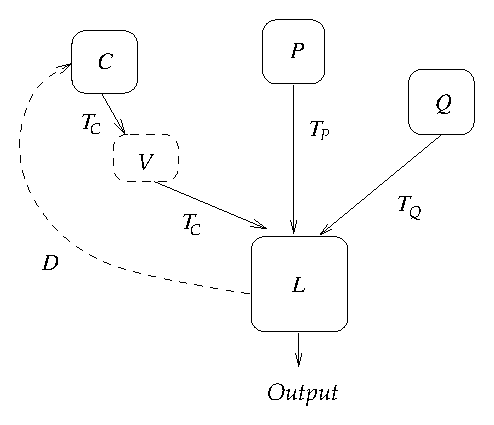
\includegraphics{Figures/tmstruct.eps}
& 
\hspace{-10mm}
$
\begin{array}[b]{rcl}
P &:& \text{Policy}\\
C &:& \text{Certificates}\\
Q &:& \text{Authorization Query}\\
V &:& \text{Certificate Validation}\\
L &:& \text{Authorization Mechanism}\\
T_P &:& \text{Policy Compilation}\\
T_C &:& \text{Credential Encoding}\\
T_Q &:& \text{Query Compilation}\\
D &:& \text{Distributed Certificate Discovery}\\
\end{array}
$
\end{tabular}
\vspace{2mm}
\end{fpfig}
}

% Figures Related to SpartanRPC and Sprocket
%%%%%%%%%%%%%%%%%%%%%%%%%%%%%%%%%%%%%%%%%%%%

\newcommand{\snowcloudfig}
{
\begin{fpfig}[t]
{A Snowcloud Sensor Node (L,C) and Harvester Device (R).}
{figure-snowcloud}
\vspace{3mm}
\begin{center}
\begin{tabular}{ccc}
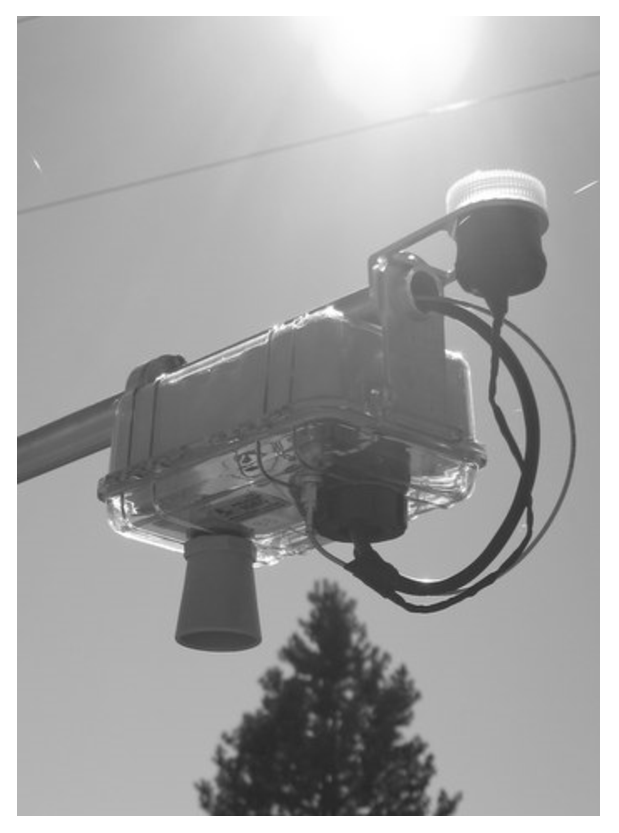
\includegraphics[scale=.35]{Figures/brainbox.eps}
& 
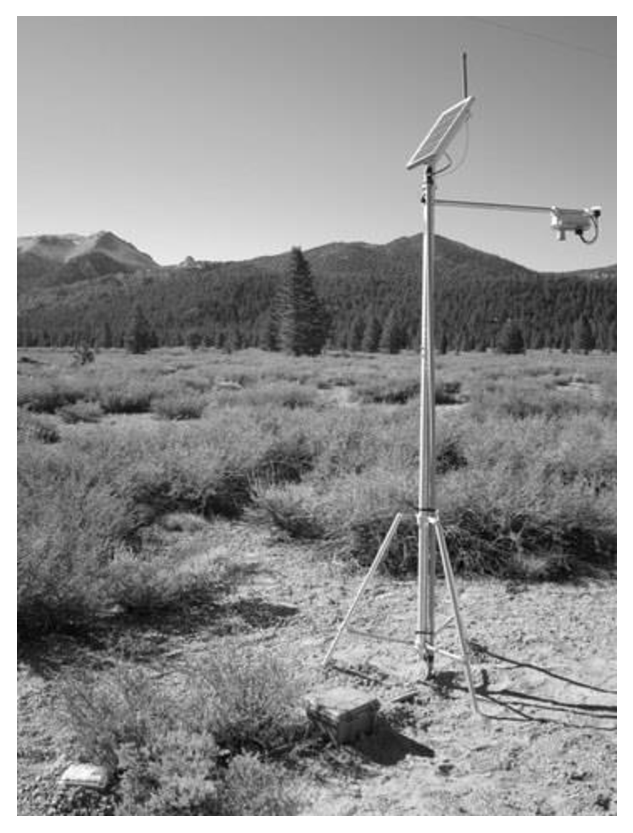
\includegraphics[scale=.35]{Figures/tower.eps} 
&
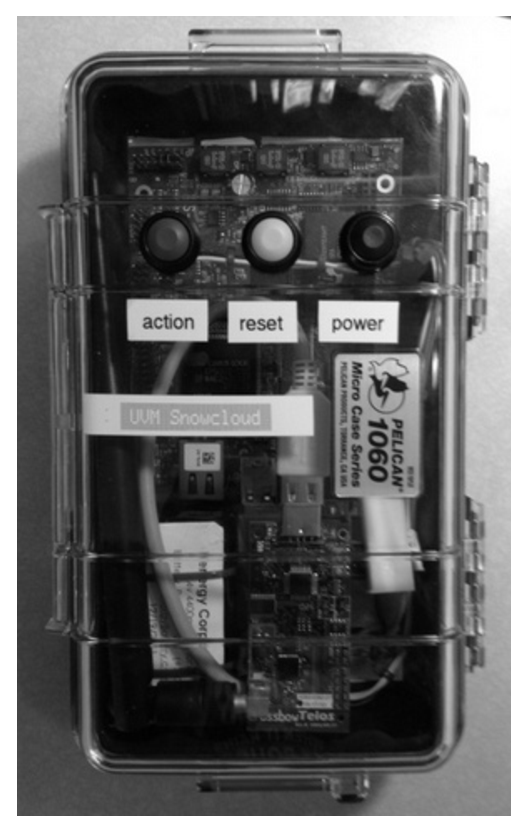
\includegraphics[scale=.35]{Figures/harvester.eps} 
\end{tabular}
\end{center}
\end{fpfig}
}

% Figures Related to nesT and Scalaness
%%%%%%%%%%%%%%%%%%%%%%%%%%%%%%%%%%%%%%%

\newcommand{\syntaxfig}
{
\begin{fpfig*}[t]{Program Syntax of nesT}{figure-syntax}
\figsize
$$
\begin{array}{lc@{\ }l@{\hspace{-5mm}}r}
\s, \t & \defassign &
   \TVAR\ \mid \top \mid \intone\ \mid \inttwo \mid \intt \mid \undefv \mid & \textit{types} \\
       &            &
   \lc\tbindvec{\fdname}{\t}\rc \mid \t \idx{} \mid \t \kwstar \\

e      & \defassign &
    v \mid \lvalue \mid e \op e \mid \castto{\t}{e} \mid \fname\blok{} \mid \lvalue = e \mid \mid \& \lvalue \mid e \rhd e \mid & \textit{expressions} \\
       &            &
    \kwif\ (e)\  e\ \kwelse\ e \mid \kwwhile\ (e)\  e \mid e; e \mid \kwpost\ \fname\blok{\,} &\\

\lvalue & \defassign &
    x \mid e\idx{e} \mid e.\fdname \mid \kwstar e & \textit{l-values} \\

v       & \defassign &
    \neight \mid \nsixtn \mid \undefv & \textit{base values} \\
% \mv &\defassign& v \mid  
%  \arr{\vect \bn} \mid \lc \vect{\fdname = \bn} \rc & 
%\textit{values in memory}\\ 

\mathit{op} & \defassign &
    + \mid \kwstar \mid \texttt{\&\&} \mid \texttt{==} \mid \,\ldots & \textit{operations} \\

\id         & \defassign &
    \fname \mid x & \textit{identifiers} \\

c           & \defassign & \fname(\vpdecl\,) : \t = \{ e \}& \textit{command definition}\\

s           & \defassign & \fname(\vpdecl\,) : \t & \textit{command signature}\\

d           & \defassign &
    \xlet{\t}{x}{e} \mid \xlet{\t}{x}{\arr{\vect{e}}} \mid \xlet{\t}{x}{\lc \defvec{\fdname}{e} \rc} \mid c & \textit{declarations} \\

\tpdecl     & \defassign & \subtvec{\TVAR}{\t} & \textit{type parameters} \\

\vpdecl     & \defassign & \tbindvec{\VAR}{\t} & \textit{value parameters} \\

\imports    & \defassign & \vect{s} & \textit{imports} \\

\exports    & \defassign & \vect{c} & \textit{exports} \\

\exportsty  & \defassign & \vect{s} & \textit{export signatures} \\

\mu         & \defassign &
    \margs{\tpdecl; \vpdecl}\lc  \imports; \decls \exports \rc  & \textit{module definitions}\\

\jmodtcat   & \defassign &
    \margs{\tpdecl; \vpdecl}\lc \imports; \exportsty \rc & \textit{module signatures}

\end{array} 
$$
\end{fpfig*}
}


\newcommand{\semanticssyntaxfig}
{ 
\begin{fpfig*}[t]{Syntactic Definitions for Dynamic Configurations}{figure-semanticssyntax}
\figsize
$$
\begin{array}{rcl@{\!\!}r}
\pi        & \defassign & \bn \mid \circ & \textit{l/r tags} \\
\kappa     & \defassign & \cval{\pi}{\mv} & \textit{dynamic objects}\\ 
\lvalue    & \defassign & \cdots \mid \cval{\bn}{\mv} \\
e          & \defassign & \cdots \mid \kappa \\
\mv        & \defassign & v \mid \bn \mid \arr{\vect{\kappa}} \mid \lc \defvec{\fdname}{\kappa} \rc &  \textit{dynamic values}\\ 
\flash     & \defassign & \tdefvec{\fname}{\t}{\blok{e}} & \textit{codebase} \\
\blockmem  & \defassign & \tdefvec{\blockno}{\t}{\mv} & \textit{memory} \\
%\rv & \defassign & \lb \mem,v\rb & \textit{runtime values} \\ 
%e & \defassign & \cdots \mid \rv & \textit{runtime expressions} \\ 
\envletter & \defassign & \context{}{} \mid \envletter; e \mid \kappa \idx{E} \mid E\idx{e} \mid E.\fdname  \mid   \kappa = \envletter \mid \envletter = e \mid a \castto{\t}{\envletter} \mid & \textit{evaluation\ contexts}\\
           &            & \kwstar \envletter \mid \&\envletter \mid \envletter \ \emph{op} \ e\ \mid \kappa\ \emph{op}\ \envletter \mid \kwif\ (\envletter)\ e\ \kwelse\ e\ \mid \kwwhile\ (E)\  e  \\ 
%{D} & \defassign & 
%    \xlet{\t}{x}{E} \mid 
%    \xlet{\t}{x}{\arr{\vect{\kappa}; E; \vect{e}}} \mid  & \textit{decl evaluation contexts}\%\  
% && \xlet{\t}{x}{\lc \defvec{f}{\kappa}; f = E; \defvec{f}{e}} \rc  \\ 
\ell       & \defassign & \bootseq{\vect{d}} \mid \runseq{e} & \textit{run levels} \\
%\\
%& & 
% \tlet{t}{\t}{E}; \vect{\decl} \mid \xlet{\t}{x}{E}; \vect{\decl}
%\\
%\lenvletter & \defassign & m\idx{E} \mid E.\fdname 
% \mid \kwstar E & \textit{evaluation lcontexts}
\end{array}
$$
\end{fpfig*}
}


\newcommand{\coresemanticsfig}
{\begin{fpfig*}[t]{Dynamic Semantics of Selected Expressions}{figure-coresemantics}
\figsize
\begin{mathpar}
\inferrule[ArrIdx]
{}
{ \blockmem, \cval{\bn}{\arr{\vect{\kappa}}}\idx{\cval{\pi}{n}} \compute \blockmem, \kappa_n}

%\inferrule[Select]
%{}
%{ \blockmem, \cval{\bn}{\lc \vect{\fdname} = \vect{\kappa} \rc}.\fdname_n \compute \blockmem,% 
% \kappa_n}
%
\inferrule[Star]
{}
{\blockmem, \kwstar\cval{\pi}{\bn} \compute \blockmem, \cval{\bn}{\blockmem(\bn)}}

\inferrule[AddrOf]
{}
{\blockmem, \&\cval{\bn}{\mv} \compute \blockmem, \cval{\circ}{\bn}}

\inferrule[Cast]
{}
{ 
\blockmem, \castto{\t}{\kappa} \compute 
   \docast{\t}{\kappa}{\blockmem}
}

\inferrule[Assign]
{}
{\blockmem, \cval{\bn}{\mv_1} = \cval{\pi}{\mv_2} \compute \blockmem[\bn \mapsto \mv_2], 
 \cval{\pi}{\mv_2}}

%\inferrule[BinaryOp]
%{\fundef{opsem}(\mathit{op}, \mv_1, \mv_2) = \mv}
%{\blockmem, \cval{\pi_1}{\mv_1}\ \mathit{op}\ \cval{\pi_2}{\mv_2} \compute 
%  \blockmem, \cval{\circ}{\mv}}
%
\inferrule[Call]
{\flash(\fname) = \blok{e}}
{\blockmem, \fname() \compute \blockmem, e}

%\inferrule[Alloc]
%{}
%{\blockmem, \kwmalloc (\tau) \compute \funalloc(\tau,\blockmem)}
%
%\inferrule[Type]
%{}
%{\blockmem, \tau \compute \blockmem \uplus \lc \bn : \typet{\tau} = \tau\rc, \bn}
%
\inferrule[Int]
{}
{\blockmem, n \compute \blockmem, \cval{\circ}{n}}

%\inferrule[Null]
%{}
%{\blockmem, \undefv \compute \blockmem, \cval{\circ}{\undefv}}
%
%\inferrule[IfTrue]
%{n \ne 0}
%{\blockmem, \kwif\ (\cval{\pi}{n})\  e_1\ \kwelse\ e_2  \compute \blockmem, e_1 }
%
%\inferrule[IfFalse]
%{}
%{\blockmem, \kwif\ (\cval{\pi}{0})\  e_1\ \kwelse\ e_2  \compute \blockmem, e_2 }
%
%\inferrule[Sequence]
%{}
%{ \blockmem, \bn; e  \compute  \blockmem, e }
%
\inferrule[While]
{}
{ \blockmem, \kwwhile\ (e_1)\  e_2 \compute  \blockmem, \kwif(e_1)\ e_2; \kwwhile\ (e_1)\  e_2\ \kwelse\ \undefv}

\inferrule[Context]
{\blockmem,    e \compute  \blockmem, e'}
{\blockmem,    \context{E}{e} \compute  \blockmem,  \context{E}{e'}
}
\end{mathpar}
\end{fpfig*}
}

\newcommand{\lvaluesemanticsfig}
{
\begin{figure}[t]
\figurebox{

\begin{mathpar}
\inferrule[AssignCong]
{\blockmem, \lvalue \lcompute \blockmem', \lvalue'}
{\blockmem, \lvalue = e \compute \blockmem', \lvalue' = e}

\inferrule[ArrIdx]
{
\blockmem(\bn') = n \\ \blockmem(\bn)(n) = \bn_n
}
{ \blockmem, \bn\idx{\bn'} \lcompute \blockmem, \bn_n}

\inferrule[Select]
{\blockmem(\bn)(\fdname) = \bn_\fdname}
{\blockmem, \bn.\fdname \lcompute \blockmem, \bn_\fdname}

\inferrule[Star]
{}
{\blockmem, \kwstar\bn \lcompute \blockmem, \blockmem(\bn)}

\inferrule[ELContext]
{\blockmem,    e \compute  \blockmem, e'}
{\blockmem,    \lenv{}{e} \lcompute  \blockmem,  \lenv{}{e'}}

\inferrule[LEContextV]
{\blockmem,    \lenv{}{\bn'} \lcompute  \blockmem, \bn}
{\blockmem,    \env{}{\lenv{}{\bn'}} \compute  \blockmem,
  \env{}{\blockmem(\bn)}}

\inferrule[LEContextE]
{\blockmem,    \lenv{}{e} \lcompute  \blockmem, \lenv{}{e'} }
{\blockmem,    \env{}{\lenv{}{e}} \compute  \blockmem,  \env{}{\lenv{}{e'}}}
\end{mathpar}
}
\caption{Dynamic Semantics of lvalues} 
\label{fig:nest-lvaluesemantics}
\label{figure-lvaluesemantics}
\end{figure}
}

\newcommand{\modsemanticsfig}
{
\begin{fpfig*}[t]{Dynamic Semantics of Module Construction}{figure-modsemantics}
\figsize
\begin{mathpar}
\inferrule[Mod]
{ v = \margs{\tpdecl, \vpdecl}\lc \imports; \vect{\decl}; \exports \rc}
{\blockmem, v \compute \blockmem \uplus \lc \bn : \modty(v) = v \rc, \bn}


\inferrule[ModInst]
{
\blockmem(m) = \margs{\vect{t \subtype \t'}; \vect{x : \tau''}
   }\lc  \imports; \vect{\decl}; \exports \rc\\
\serialize(\vect{x}, \t''[\vect{\t}/\vect{t}], \vect{\bn}) = \vect{\decl'}
}
{\blockmem,  \bn \margs{\vect{\t},\vect{\bn}}  \compute 
  \blockmem, \margs{}\lc\imports; \vect{\decl} @ \vect{\decl'}; \exports \rc[\vect{\t}/\vect{t}]
}

\inferrule[ModWire]
{
\blockmem(\bn_1) = \margs{}\lc  \imports_1; \vect{\decl_1}; \exports_1 \rc\\
\blockmem(\bn_2) = \margs{}\lc  \imports_2; \vect{\decl_2}; \exports_2 \rc\\\\
\vect{\decl_3} = \exports_2 \restr \dom(\imports_1) \\
\imports' = (\imports_1 \maploosemerge \imports_2) / \exports_2
}
{\blockmem, \bn_1 \modwire \bn_2 \compute \blockmem, 
  \margs{}
  \lc \imports' ; \vect{\decl_2} @ \vect{\decl_3} @ \vect{\decl_1}; \exports_1 \rc} 

\inferrule[Validate]
{\blockmem(\bn) = \margs{}\lc\ ; \vect{\decl}; \exports\rc }
{\blockmem, \kwrun\ \bn \compute \blockmem, \undefv}
\end{mathpar}
\end{fpfig*}
}

\newcommand{\subjudgefig}
{
\begin{fpfig*}[t]{Subtyping Rules}{figure-subjudge}
\figsize
\begin{mathpar}
\inferrule[ReflS]
{}
{\subjudge{\tpdecl}{\tau}{\tau}}

\inferrule[TopS]
{}
{\subjudge{\tpdecl}{\tau}{\top}}

\inferrule[TransS]
{\subjudge{\tpdecl}{\tpdecl(t)}{\tau}}
{\subjudge{\tpdecl}{t}{\tau}}

\inferrule[UintS]
{}
{\subjudge{\tpdecl}{\intone}{\inttwo \subtype \intt}}

\inferrule[FnBodyS]
{\subjudge{\tpdecl}{\t_1}{\t_2}}
{\subjudge{\tpdecl}{\blok{\t_1}}{\blok{\t_2}}}

\inferrule[StructS]
{\tpdecl \vdash \vect{\t_1 \subtype \t_3}}
{\subjudge{\tpdecl}{\lc\vect{\fdname_1 : \t_1}
  \uplus \vect{\fdname_2 : \t_2} \rc}{\lc\vect{\fdname_1 : \t_3}\rc}}
%
%\inferrule[TypeS]
%{\subjudge{\tpdecl}{\tau}{\tau'}}
%{\subjudge{\tpdecl}{\typet{\tau}}{\typet{\tau'}}}
%
%\inferrule[ExistsS]
%{\subjudge{\tpdecl; t\subtype \tau}{\tau_0 }{\tau_1}}
%{\subjudge{\tpdecl}{(\texist{t \subtype \tau}{\tau_0})} 
%{(\texist{t \subtype\tau}{\tau_1})}}
%
%\inferrule[ModS]
%{
%\subjudge{\tpdecl[\tpdecl_0]}{\vpdecl_2}{\vpdecl_1} \\ 
%\subjudge{\tpdecl[\tpdecl_0]}{\imports_2}{\imports_1} \\ 
%\subjudge{\tpdecl[\tpdecl_0]}{\exportsty_1}{\exportsty_2}
%}
%{\subjudge{\tpdecl}
% {\margs{\tpdecl_0, \vpdecl_1 }\lc \imports_1, \exportsty_1 \uplus \exportsty \rc}
% {\margs{\tpdecl_0, \vpdecl_2 }\lc \imports_2 \uplus \imports, \exportsty_2 \rc}}
\end{mathpar}
\end{fpfig*}
}

\newcommand{\selectsubjudgefig}
{
\begin{fpfig*}[t]{Selected Subtyping Rules}{figure-selectsubjudge}
\figsize
\begin{mathpar}
\inferrule[UintS]
{}
{\subjudge{\tpdecl}{\intone}{\inttwo \subtype \intt}}

\inferrule[StructS]
{}
{\subjudge{\tpdecl}{\lc\vect{\fdname_1 : \t_1}
  \uplus \vect{\fdname_2 : \t_2} \rc}{\lc\vect{\fdname_1 : \t_1}\rc}}

\inferrule[ModS]
{
\subjudge{\tpdecl[\tpdecl_0]}{\vpdecl_2}{\vpdecl_1} \\ 
\subjudge{\tpdecl[\tpdecl_0]}{\imports_2}{\imports_1} \\ 
\subjudge{\tpdecl[\tpdecl_0]}{\exportsty_1}{\exportsty_2}
}
{\subjudge{\tpdecl}
 {\margs{\tpdecl_0, \vpdecl_1 }\lc \imports_1, \exportsty_1 \uplus \exportsty \rc}
 {\margs{\tpdecl_0, \vpdecl_2 }\lc \imports_2 \uplus \imports, \exportsty_2 \rc}}
\end{mathpar}
\end{fpfig*}
}

\newcommand{\coretypingfig}
{
\begin{fpfig*}[t]{Typing Rules for Selected Expressions}{figure-coretyping}
\figsize
\begin{mathpar}
%\inferrule[SequenceT]
%{\tenv,\tpdecl \vdash e_0 : \texist{\tpdecl_0}{\s_0} \\ 
%\tenv,\tpdecl \vdash e_1 : \texist{\tpdecl_1}{\s_1}}
%{\tenv,\tpdecl \vdash e_0 ; e_1 : \texist{\tpdecl_0 \maploosemerge \tpdecl_1}{\s_1}}
%
\inferrule[CastT]
{\tenv,\tpdecl \vdash e : \t \\ T \vdash \compatible{\t}{\s}}
{\tenv,\tpdecl \vdash (\s) e : \s}

\inferrule[CallT]
{\tenv,\tpdecl \vdash \fname : \s\\
\tpdecl  \vdash \s \promote \blok{\t}}
{\tenv,\tpdecl \vdash \fname() : \t}

%\inferrule[CondT]
%{\tenv, \tpdecl \vdash e_1 : \s_1 \\ 
% \tenv, \tpdecl \vdash e_2 : \s_2 \\
% \tenv, \tpdecl \vdash e_3 : \s_3 \\
% \tpdecl \vdash \s_1 \subtype \intt \\  
% \tpdecl \vdash \s_2 \promote \undefv \\  
% \tpdecl \vdash \s_3 \promote \undefv
% }
% {\tenv,\tpdecl \vdash \eite{e_1}{e_2}{e_3} : \undefv}
%
\inferrule[AssignT]
{\tenv, \tpdecl \vdash e_1 : \s_1 \\ 
 \tenv, \tpdecl \vdash e_2 : \s_2 \\
 \tpdecl \vdash \s_2 \subtype \s_1 
}
{\tenv,\tpdecl \vdash e_1 = e_2 : \s_1}

%\inferrule[AllocT]
%{}
%{\tenv,\tpdecl \vdash \kwmalloc(\t) : \t\kwstar}
%
\inferrule[StarT]
{
 \tenv,\tpdecl \vdash e : \s \\ 
 \tpdecl \vdash \s \promote \t\kwstar 
}
{\tenv,\tpdecl \vdash \kwstar e : \t}

\inferrule[NameT]
{\tenv(\identifier) = \t}
{\tenv,\tpdecl \vdash \identifier : \t}

\inferrule[IndexT]
{
 \tenv, \tpdecl \vdash e_1 : \s_1 \\ 
 \tenv, \tpdecl \vdash e_2 : \s_2 \\
 \tpdecl \vdash \s_1 \promote \t \idx{} \\
 \tpdecl \vdash \s_2 \subtype \intt 
}
{\tenv,\tpdecl \vdash e_1 \idx{e_2} : \t}

%\inferrule[ArrayIncrT]
%{
% \tenv, \tpdecl \vdash e_1 : \s_1 \\ 
% \tenv, \tpdecl \vdash e_2 : \s_2 \\
% \tpdecl \vdash \s_1 \promote \t \idx{} \\
% \tpdecl \vdash \s_2 \subtype \intt 
%}
%{\tenv,\tpdecl \vdash e_1 \pluseq e_2 : \t \idx{}}
%\inferrule[BlockT]
%{\tenv,\tpdecl \vdash e : \texist{\tpdecl'}{\s}}
%{\tenv,\tpdecl \vdash \blok{e} : \texist{\tpdecl'}{\blok{\s}}}
%
\end{mathpar}
\end{fpfig*}
}

\newcommand{\declmodtypingfig}{
\begin{fpfig*}[t]{Selected Declaration and Module Typing Rules}{figure-declmodtyping}
\begin{mathpar}
% \xlet{\t}{x}{e} \mid \xlet{\t}{x}{\arr{\vect{e}}} \mid \xlet{\t}{x}{\lc \defvec{\fdname}{e} \rc} \mid \fname : \t =  \blok{e}
\inferrule[DeclsNoneT]
{ }
{\tenv, \tpdecl \vdash \varnothing : \varnothing}

\inferrule[DeclsSomeT]
{\tenv, \tpdecl \vdash d \Rightarrow (x : \t) \\ (x : \t) \tenv, \tpdecl \vdash \vect{d} : \tenv'}
{\tenv, \tpdecl \vdash d \vect{d} : (x : \t) \tenv'}

\inferrule[DeclBaseT]
{\tenv, \tpdecl \vdash e : \t}
{\tenv, \tpdecl \vdash \xlet{\t}{x}{e} \Rightarrow x : \t}

%\inferrule[DeclArrayT]
%{\tenv, \tpdecl \vdash \vect{e} : \t}
%{\tenv, \tpdecl \vdash \xlet{\t\idx{}}{x}{\arr{\vect{e}}} \Rightarrow x : \t \idx{}}
%
%\inferrule[DeclStructT]
%{\tenv, \tpdecl \vdash \vect{e} : \vect{\t}}
%{\tenv, \tpdecl \vdash \xlet{\t}{x}{\lc \defvec{\fdname}{e} \rc} \Rightarrow 
%  x : \lc \tbindvec{\fdname}{\t} \rc}
%
\inferrule[DeclFunT]
{\tenv, \tpdecl \vdash e : \t}
{\tenv, \tpdecl \vdash \fname : \blok{\t} = \blok{e} \Rightarrow 
  \fname : \blok{\t}}

\inferrule[ModuleT]
{ 
\imports @ \vpdecl, \tpdecl \vdash \vect{d} : \tenv \\
\tenv @ \imports @ \vpdecl, \tpdecl \vdash \exports : \exportsty 
}
{\margs{\tpdecl, \vpdecl}\lc \imports; \vect{\decl}; \exports \rc : 
  \margs{\tpdecl, \vpdecl}\lc \imports; \exportsty \rc}
\end{mathpar}
\end{fpfig*}
}

\newcommand{\modtypingfig}{
\begin{fpfig*}[t]{Module Typing Rule}{figure-modtyping}
\begin{mathpar}
\inferrule[ModT]
{
\vpdecl\, @\, \imports, \tpdecl \vdash \vect{d} : \tenv\\
\vpdecl\, @\, \imports\, @\, \tenv, \tpdecl \vdash \exports : \exportsty
}
{
\margs{\tpdecl; \vpdecl} 
\lc  
  \imports;
  \vect{d};
  \exports
\rc
:  
\margs{\tpdecl; \vpdecl} 
\lc  
  \imports,
  \exportsty
\rc
}
\end{mathpar}
\end{fpfig*}
}

\newcommand{\modoptypingfig}{
\begin{fpfig*}[t]{Module Typing Rules}{figure-modtyping}
\figsize
\begin{mathpar}
\inferrule[ModT]
{
\vpdecl_0[\imports], 
\tpdecl_1[\tpdecl_0] \vdash \exports
}
{
\tenv_1, \tpdecl_1 \vdash \margs{\tpdecl_0; \vpdecl_0} 
\lc  
  \imports,
  \exports
\rc
:  
\modty{(\margs{\tpdecl_0; \vpdecl_0} 
\lc  
  \imports,
  \exports
\rc)}
}

\inferrule[ModInstT]
{
\tenv, \tpdecl \vdash e : \texist{\tpdecl'}{\s}\\
\tenv,\tpdecl \vdash \tbindvec{e}{\texist{\tpdecl}{\s}}\\
\tpdecl'' = (\maploosemerge\vect\tpdecl) \maploosemerge \tpdecl'\\
\tpdecl \maploosemerge \tpdecl'' \vdash \s \promote
   \margs{\subtvec{t}{\t_0};\tbindvec{\fname}{\t_1}} \lc 
  \imports; \exportsty \rc \\
\tpdecl \maploosemerge \tpdecl'' \vdash \subtvec{\t}{\t_0}\\
 \vect{\texist{\tpdecl}{\s}} = \vect{\t_1}[\vect{\tau/t}] 
}
{
\tenv,\tpdecl \vdash 
e \margs{\vect{\t},\vect{e}} 
: 
\texist{\tpdecl''}{(\margs{}\lc \imports;  \exportsty \rc)
[\subnvec{\t}{t}]}
}

\inferrule[ModCompT]
{
\tenv,\tpdecl \vdash e_0 : \texist{\tpdecl_0}{\s_o}\\
\tenv,\tpdecl \vdash e_1 : \texist{\tpdecl_1}{\s_1}\\
\tpdecl' = \tpdecl_0 \maploosemerge \tpdecl_1\\
\tpdecl \maploosemerge \tpdecl' \vdash \s_0 \promote  \margs{\tpdecl_0',\vpdecl_0} \lc 
  \imports_0;   \exportsty_0 \rc \\
\tpdecl \maploosemerge \tpdecl' \vdash \s_1 \promote \margs{\tpdecl_1',\vpdecl_1} \lc 
  \imports_1;   \exportsty_1\rc }
{
\tenv,\tpdecl \vdash e_0 \modcomp e_1 : 
\texist{\tpdecl'}{\margs{\tpdecl_0' \maploosemerge \tpdecl_1', \vpdecl_0 \maploosemerge \vpdecl_1} \lc 
(\imports_0 \maploosemerge \imports_1) / \dom(\exportsty); \exportsty_0 \uplus \exportsty_1 \rc}
}

\inferrule[ValidateT]
{
\tenv, \tpdecl \vdash e : \texist{\tpdecl'}{\s} \\ 
 \tpdecl \maploosemerge \tpdecl' \vdash \s \promote  \margs{}\lc ;   \exportsty \rc \\ 
}
{\tenv,\tpdecl \vdash \kwrun\  e: \texist{\tpdecl'}{\undefv}}

\inferrule[TypedefT]
{
\tenv, \tpdecl \vdash e_0 : \texist{\tpdecl_0}{\s_0}\\
\tenv, \tpdecl[t \subtype \t] \vdash e_1 : \texist{\tpdecl_1}{\s_1}\\
\tpdecl' = \tpdecl_0 \maploosemerge \tpdecl_1 \maploosemerge [t \subtype \t] \\
\tpdecl \maploosemerge \tpdecl' \vdash \s_0 \subtype \typet{\t} 
}
{
\tenv, \tpdecl \vdash \tlet{t}{\t}{e_0}{e_1} : \texist{\tpdecl'}{\s_1}
}
\end{mathpar}
\end{fpfig*}
}

\newcommand{\configtypingfig}
{
\begin{fpfig*}[t]{Memory, Codebase, and Configuration Typing}{figure-configtyping}
\figsize
\begin{mathpar}
\inferrule[ValDef]
{v \text{ not a memory location} \\ 
 \tenv[\vect{\localname : \t}], \tpdecl \vdash v : \t' \\ 
 \subjudge{\tpdecl}{\t'}{\t}
}
{\tenv, \tpdecl, \vect{\localname : \t = \mv} \vdash v : \t}

\inferrule[ArrayM]
{\forall 0 \le i < n . \ascript(\mv(i), \exports) = \t}
{\tenv, \tpdecl, \exports \vdash \mv : \t\idx{n}}

\inferrule[StructM]
{
 \vect{\ascript(\bn, \exports)} = \vect{\t}
}
{\tenv, \tpdecl, \exports \vdash \lc 
 \vect{\fdname = \bn} \rc : \lc\vect{\fdname : \t} \rc}

\inferrule[PtrM]
{\ascript(\bn, \exports) = \t}
{\tenv, \tpdecl, \exports \vdash \bn : \t\kwstar }

\inferrule[UninitM]
{\exports(\bn) = \undefv}
{\tenv, \tpdecl, \exports \vdash \bn : \t\kwstar }

\inferrule[DefsT]
{\forall (\localname : \t = \mv) \in \exports . \tenv, \tpdecl, 
 \exports \vdash \mv : \t}
{\tenv, \tpdecl \vdash \exports}

\inferrule[Config]
{ \forall \fname() \in \tasks . \fname \in \dom(\flash) \\ 
  \varnothing, \varnothing \vdash \flash[\blockmem] \\ \varnothing, \varnothing, \flash[\blockmem] \vdash e : \texist{\tpdecl}{\s}
}
{(\flash,\tasks,\blockmem,e) : (\tpdecl, \s)}
\end{mathpar}
\end{fpfig*}
}

\newcommand{\tasksemanticsfig}
{
\begin{fpfig*}[t]{Semantics of Tasks and Configurations}{figure-tasksemantics}
\begin{mathpar}
\figsize
\inferrule[CoreStep]
{\blockmem, e  \compute \blockmem',  e'}
{\tasks, \blockmem, e  \tcompute{} \tasks, \blockmem',  e'}

\inferrule[Post]
{}
{\tasks, \blockmem,  \context{E}{\kwpost\ \fname\blok{}}  \tcompute{}
 \addt(\tasks,\fname\blok{}), \blockmem,  \context{E}{\undefv}}

\inferrule[TaskStart]
{\nextt(\tasks) = \tasks',\fname\blok{}}
{\tasks, \blockmem, \bn  \tcompute{}
  \tasks', \blockmem,  \fname\blok{}}
\end{mathpar}
\end{fpfig*}
}

\newcommand{\declsemanticsfig}
{
\begin{fpfig*}[t]{Semantics of Declarations}{figure-declsemantics}
\begin{mathpar}
\inferrule[DeclContext]
{\flash \vdash \tasks, \bm, e \compute \tasks', \bm', e'}
{\flash, \tasks, \bm, D[e] \vect{\decl} \compute \flash, \tasks', \bm', D[e'] \vect{\decl}}

\inferrule[BaseInit]
{\kappa = \cval{\bn}{\mv} \\ \bn \not\in \dom(\bm)}
{\flash, \tasks, \bm,(\xlet{\t}{x}{\cval{\pi}{\mv}}) \vect{\decl} \compute 
 \flash, \tasks, (\bn : \t = \mv)\bm, \vect{\decl}[\kappa/x]}

\inferrule[StructInit]
{\kappa = \cval{\bn}{\mv} \\ \bn \not\in \dom(\bm)}
{\flash, \tasks, \bm,(\xlet{\t}{x}{\mv}) \vect{\decl} \compute 
 \flash, \tasks, (\bn : \t = \mv)\bm, \vect{\decl}[\kappa/x]}

\inferrule[FDecl]
{}
{\flash, \tasks, \bm, (\fname : \t = \blok{e}) \vect{\decl} \compute 
 (\fname : \t = \blok{e}) \flash, \tasks, \bm, \vect{\decl}}
\end{mathpar}
\end{fpfig*}
}

\newcommand{\bootloadsemanticsfig}
{
\begin{fpfig*}[t]{Boot and Runtime Semantics}{figure-bootloadsemantics}
\begin{mathpar}
\inferrule[RunTime]
{\flash \vdash \tasks,\bm,e \compute \tasks',\bm',e'}
{\flash,\tasks,\bm,\runseq{e} \compute \flash,\tasks',\bm',\runseq{e'}}

\inferrule[BootTime]
{\flash,\tasks,\bm,\vect{d} \compute \flash',\tasks',\bm',\vect{d}'}
{\flash,\tasks,\bm,\bootseq{\vect{d}} \compute 
 \flash',\tasks',\bm',\bootseq{\vect{d}'}}

\inferrule[RunStart]
{}
{\flash,\tasks,\bm,\bootseq{\emptyset} \compute 
 \flash,\tasks,\bm,\runseq{\textrm{main}\blok{}}}
\end{mathpar}
\end{fpfig*}
}

\newcommand{\scalanesssyntaxfig}
{
\begin{fpfig*}[t]{The Syntax of DScalaness}{figure-scalanesssyntax}
$$
\begin{array}{rcl@{\hspace{3mm}}r}
\\[-4mm]%
\tt{L} & ::= & \gclass{C}{\gbounds{X}{N}}{N}{\fieldvec{T}{f};\ K\ \ttvec{M}} & \gdesc{class definitions}\\[1mm]
\tt{K} & ::= & \init{C}{\tdecls{T}{f}}{\super(\ttvec{f});\ \this.\ttvec{f}=\ttvec{f};} & \gdesc{constructors}\\[1mm]
\tt{M} & ::= & \meth{T}{m}{\tdecls{T}{x}}{\return{e};} & \gdesc{methods}\\[1mm]
\tt{e} & ::= & \tt{x} \mid \select{e}{f} \mid \send{e}{m}{\ttvec{e}} \mid \gnew{C}{\ttvec{T}}{\ttvec{e}}  \mid \cast{N}{e} \mid \mutate{\select{e}{f}}{e} \mid \tt{l} \mid  & \gdesc{expressions}\\
       &     & \jdef{x}{T}{e}{e} \mid % \jtlet{x}{\tt{T}}{e}{e} \mid \\ & & 
\jmodval \mid \jwire{\tt{e}}{\tt{e}} \mid \jinst{e}{\ttvec{e};\ttvec{e}} \mid \jimage{\tt{e}} \mid \\
       &     & \abbrvt{X(\ttvec{X})}{T}{e} \\[1mm]
\tt{T} & ::= & \tt{X} \mid \tt{N} \mid \jmodt{\tpdecl}{\jmodtcat} & \gdesc{scala level types} \\[1mm]
\tt{N} & ::= & \jinst{C}{\ttvec{T}} & \gdesc{class types}\\[1mm]
\tt{l} & ::= & \jref{\tt{p}}{N} & \gdesc{references}
\end{array}
$$
\end{fpfig*}
}

\newcommand{\jmodsemanticsfig}
{
\begin{fpfig*}[t]{DScalaness Module Semantics}{figure-jmodsemantics}
\begin{mathpar}
\inferrule[ModInst]
{
\jmodval = \margs{\subtvec{t}{\t}; \tbindvec{x}{\s}}
   \lc  \imports; \vect{\decl}; \exports \rc\\
\serialize(\vect{x}, \vect{\s}, \ttvec{l}) = \vect{\decl'}
}
{ 
 \jinst{\jmodval}{\jref{\vect{p}}{\jinst{MetaType}{\ttvec{T}}};\,\ttvec{l}}  \rightarrow 
   \margs{}\lc\imports; \vect{\decl'} @ \vect{\decl}; \exports \rc[\codt{\ttvec{T}}/\vect{t}]
}

\inferrule[ModWire]
{\imports = (\imports_1 / \dom(\exports_2)) @ \imports_2 \\
 \vect{d} = \vect{d}_2 @ \restrict{\exports_2}{\dom(\imports_1)} 
}
{\jwire{\margs{\tpdecl_1,\vpdecl_1} \lc  \imports_1; \vect{d}_1; \exports_1 \rc}
       {\margs{\tpdecl_2,\vpdecl_2} \lc  \imports_2; \vect{d}_2; \exports_2 \rc}\\\\
 \rightarrow\\\\
   \margs{\tpdecl_1 \maploosemerge \tpdecl_2,\vpdecl_1 \maploosemerge \vpdecl_2} 
    \lc  \imports; \vect{\decl} \maploosemerge \vect{\decl}_1; \exports_1 \rc
}

\inferrule[ModImage]
{}
{\jimage{(\margs{}\lc ; \vect{d}; \exports \rc)} \rightarrow \margs{}\lc ; \vect{d}; \exports \rc}
\end{mathpar}
\end{fpfig*}
}

\newcommand{\scalanesstypingfig}
{
\begin{fpfig*}[t]{DScalaness Module Typing Rules}{figure-scalanesstyping}
\begin{mathpar}
\inferrule[ModT]
{\jmodval : \jmodtcat \text{\ in\ nesT\ type\ checking}}
{\Gamma \vdash \jmodval : \jmodt{\varnothing}{\jmodtcat}}

\inferrule[ModInstT]
{\Gamma \vdash \tt{e} : \jmodt{\varnothing}{\margs{\vect{t} \subtype \vect{\t}_1; 
 \vect{x} \subtype \vect{\t}_2} \lc 
  \imports; \exportsty \rc}\\
 \Gamma \vdash \ttvec{e}_1 : \jinst{MetaType}{\ttvec{T}_1}\\
 \Gamma \vdash \ttvec{e}_2 : \ttvec{T}_2 \\
 \vdash \codt{\ttvec{T}_1} \subtype \vect{\t}_1\\
 \vdash \codt{\ttvec{T}_2} \subtype \vect{\t}_2
}
{\Gamma \vdash \jinst{e}{\ttvec{e}_1; \ttvec{e}_2} : \jmodt{\vect{t}\subtype \codt{\ttvec{T}_1}}{\margs{} \lc 
  \imports; \exportsty \rc} }

\inferrule[ModWireT]
{
 \Gamma \vdash \tt{e}_1 : \jmodt{\tpdecl_1}{\margs{}\lc\imports_1; \exportsty_1 \rc}\\
 \Gamma \vdash \tt{e}_2 : \jmodt{\tpdecl_2}{\margs{}\lc\imports_2; \exportsty_2 \rc} \\
 \imports = (\imports_1 / \dom(\exportsty_2)) @ \imports_2 \\
}
{\Gamma \vdash \jwire{\tt{e}_1}{\tt{e}_2} : 
 \jmodt{\tpdecl_1 \maploosemerge \tpdecl_2}{\margs{}\lc\imports; \exportsty_1 \rc}}

\inferrule[ModImageT]
{
  \Gamma \vdash \tt{e} : \jmodt{\tpdecl}{\margs{}\lc \imports; \exportsty \rc} \\
  \text{main}() : \t \in \exportsty
}
{
  \Gamma \vdash \jimage{\tt{e}} : \jmodt{\tpdecl}{\margs{}\lc \imports; \exportsty \rc}
}
\end{mathpar}
\end{fpfig*}
}
